\chapter{Tuples}
\label{tuplechap}

\section{Tuples are immutable}
\index{tuple}
\index{type!tuple}
\index{sequence}

A tuple is a sequence of values.  The values can be any type, and
they are indexed by integers, so in that respect tuples are a lot
like lists.  The important difference is that tuples are immutable.
\index{mutability}
\index{immutability}

Syntactically, a tuple is a comma-separated list of values:

\begin{verbatim}
>>> t = 'a', 'b', 'c', 'd', 'e'
\end{verbatim}
%
Although it is not necessary, it is common to enclose tuples in
parentheses:
\index{parentheses!tuples in}

\begin{verbatim}
>>> t = ('a', 'b', 'c', 'd', 'e')
\end{verbatim}
%
To create a tuple with a single element, you have to include a final
comma:
\index{singleton}
\index{tuple!singleton}

\begin{verbatim}
>>> t1 = 'a',
>>> type(t1)
<type 'tuple'>
\end{verbatim}
%
A value in parentheses is not a tuple:

\begin{verbatim}
>>> t2 = ('a')
>>> type(t2)
<type 'str'>
\end{verbatim}
%
Another way to create a tuple is the built-in function {\tt tuple}.
With no argument, it creates an empty tuple:
\index{tuple function}
\index{function!tuple}

\begin{verbatim}
>>> t = tuple()
>>> print t
()
\end{verbatim}
%
If the argument is a sequence (string, list or tuple), the result
is a tuple with the elements of the sequence:

\begin{verbatim}
>>> t = tuple('lupins')
>>> print t
('l', 'u', 'p', 'i', 'n', 's')
\end{verbatim}
%
Because {\tt tuple} is the name of a built-in function, you should
avoid using it as a variable name.

Most list operators also work on tuples.  The bracket operator
indexes an element:
\index{bracket operator}
\index{operator!bracket}

\begin{verbatim}
>>> t = ('a', 'b', 'c', 'd', 'e')
>>> print t[0]
'a'
\end{verbatim}
%
And the slice operator selects a range of elements.
\index{slice operator}
\index{operator!slice}
\index{tuple!slice}
\index{slice!tuple}

\begin{verbatim}
>>> print t[1:3]
('b', 'c')
\end{verbatim}
%
But if you try to modify one of the elements of the tuple, you get
an error:
\index{exception!TypeError}
\index{TypeError}
\index{item assignment}
\index{assignment!item}

\begin{verbatim}
>>> t[0] = 'A'
TypeError: object doesn't support item assignment
\end{verbatim}
%
You can't modify the elements of a tuple, but you can replace
one tuple with another:

\begin{verbatim}
>>> t = ('A',) + t[1:]
>>> print t
('A', 'b', 'c', 'd', 'e')
\end{verbatim}
%

\section{Tuple assignment}
\label{tuple.assignment}
\index{tuple!assignment}
\index{assignment!tuple}
\index{swap pattern}
\index{pattern!swap}

It is often useful to swap the values of two variables.
With conventional assignments, you have to use a temporary
variable.  For example, to swap {\tt a} and {\tt b}:

\begin{verbatim}
>>> temp = a
>>> a = b
>>> b = temp
\end{verbatim}
%
This solution is cumbersome; {\bf tuple assignment} is more elegant:

\begin{verbatim}
>>> a, b = b, a
\end{verbatim}
%
The left side is a tuple of variables; the right side is a tuple of
expressions.  Each value is assigned to its respective variable.  
All the expressions on the right side are evaluated before any
of the assignments.

The number of variables on the left and the number of
values on the right have to be the same:
\index{exception!ValueError}
\index{ValueError}

\begin{verbatim}
>>> a, b = 1, 2, 3
ValueError: too many values to unpack
\end{verbatim}
%
More generally, the right side can be any kind of sequence
(string, list or tuple).  For example, to split an email address
into a user name and a domain, you could write:
\index{split method}
\index{method!split}
\index{email address}

\begin{verbatim}
>>> addr = 'monty@python.org'
>>> uname, domain = addr.split('@')
\end{verbatim}
%
The return value from {\tt split} is a list with two elements;
the first element is assigned to {\tt uname}, the second to
{\tt domain}.

\begin{verbatim}
>>> print uname
monty
>>> print domain
python.org
\end{verbatim}
%

\section{Tuples as return values}
\index{tuple}
\index{value!tuple}
\index{return value!tuple}
\index{function, tuple as return value}

Strictly speaking, a function can only return one value, but
if the value is a tuple, the effect is the same as returning
multiple values.  For example, if you want to divide two integers
and compute the quotient and remainder, it is inefficient to
compute {\tt x/y} and then {\tt x\%y}.  It is better to compute
them both at the same time.
\index{divmod}

The built-in function {\tt divmod} takes two arguments and
returns a tuple of two values, the quotient and remainder.
You can store the result as a tuple:

\begin{verbatim}
>>> t = divmod(7, 3)
>>> print t
(2, 1)
\end{verbatim}
%
Or use tuple assignment to store the elements separately:
\index{tuple assignment}
\index{assignment!tuple}

\begin{verbatim}
>>> quot, rem = divmod(7, 3)
>>> print quot
2
>>> print rem
1
\end{verbatim}
%
Here is an example of a function that returns a tuple:

\begin{verbatim}
def min_max(t):
    return min(t), max(t)
\end{verbatim}
%
{\tt max} and {\tt min} are built-in functions that find
the largest and smallest elements of a sequence.  \verb"min_max"
computes both and returns a tuple of two values.
\index{max function}
\index{function!max}
\index{min function}
\index{function!min}


\section{Variable-length argument tuples}
\index{variable-length argument tuple}
\index{argument!variable-length tuple}
\index{gather}
\index{parameter!gather}
\index{argument!gather}

Functions can take a variable number of arguments.  A parameter
name that begins with {\tt *} {\bf gathers} arguments into
a tuple.  For example, {\tt printall}
takes any number of arguments and prints them:

\begin{verbatim}
def printall(*args):
    print args
\end{verbatim}
%
The gather parameter can have any name you like, but {\tt args} is
conventional.  Here's how the function works:

\begin{verbatim}
>>> printall(1, 2.0, '3')
(1, 2.0, '3')
\end{verbatim}
%
The complement of gather is {\bf scatter}.  If you have a
sequence of values and you want to pass it to a function
as multiple arguments, you can use the {\tt *} operator.
For example, {\tt divmod} takes exactly two arguments; it
doesn't work with a tuple:

% removing this because we haven't seen optional parameters yet
%You can combine the gather operator with required and positional
%arguments:

%%\begin{verbatim}
%def pointless(required, optional=0, *args):
%    print required, optional, args
%\end{verbatim}
%\afterverb
%
%Run this function with 1, 2, 3 and 4 or more arguments and
%make sure you understand what it does.
\index{scatter}
\index{argument scatter}
\index{TypeError}
\index{exception!TypeError}

\begin{verbatim}
>>> t = (7, 3)
>>> divmod(t)
TypeError: divmod expected 2 arguments, got 1
\end{verbatim}
%
But if you scatter the tuple, it works:

\begin{verbatim}
>>> divmod(*t)
(2, 1)
\end{verbatim}
%
\begin{exercise}

Many of the built-in functions use
variable-length argument tuples.  For example, {\tt max}
and {\tt min} can take any number of arguments:
\index{max function}
\index{function!max}
\index{min function}
\index{function!min}

\begin{verbatim}
>>> max(1,2,3)
3
\end{verbatim}
%
But {\tt sum} does not.
\index{sum function}
\index{function!sum}

\begin{verbatim}
>>> sum(1,2,3)
TypeError: sum expected at most 2 arguments, got 3
\end{verbatim}
%
Write a function called {\tt sumall} that takes any number
of arguments and returns their sum.

\end{exercise}


\section{Lists and tuples}
\index{zip function}
\index{function!zip}

{\tt zip} is a built-in function that takes two or more sequences and
``zips'' them into a list of tuples where each tuple contains one
element from each sequence.  In Python 3, {\tt zip} returns an iterator
of tuples, but for most purposes, an iterator behaves like a list.
\index{Python 3}

This example zips a string and a list:

\begin{verbatim}
>>> s = 'abc'
>>> t = [0, 1, 2]
>>> zip(s, t)
[('a', 0), ('b', 1), ('c', 2)]
\end{verbatim}
%
The result is a list of tuples where each tuple contains
a character from the string and the corresponding element from
the list.
\index{list!of tuples}

If the sequences are not the same length, the result has the
length of the shorter one.

\begin{verbatim}
>>> zip('Anne', 'Elk')
[('A', 'E'), ('n', 'l'), ('n', 'k')]
\end{verbatim}
%
You can use tuple assignment in a {\tt for} loop to traverse a list of
tuples:
\index{traversal}
\index{tuple assignment}
\index{assignment!tuple}

\begin{verbatim}
t = [('a', 0), ('b', 1), ('c', 2)]
for letter, number in t:
    print number, letter
\end{verbatim}
%
Each time through the loop, Python selects the next tuple in
the list and assigns the elements to {\tt letter} and 
{\tt number}.  The output of this loop is:
\index{loop}

\begin{verbatim}
0 a
1 b
2 c
\end{verbatim}
%
If you combine {\tt zip}, {\tt for} and tuple assignment, you get a
useful idiom for traversing two (or more) sequences at the same
time.  For example, \verb"has_match" takes two sequences, {\tt t1} and
{\tt t2}, and returns {\tt True} if there is an index {\tt i}
such that {\tt t1[i] == t2[i]}:
\index{for loop}

\begin{verbatim}
def has_match(t1, t2):
    for x, y in zip(t1, t2):
        if x == y:
            return True
    return False
\end{verbatim}
%
If you need to traverse the elements of a sequence and their
indices, you can use the built-in function {\tt enumerate}:
\index{traversal}
\index{enumerate function}
\index{function!enumerate}

\begin{verbatim}
for index, element in enumerate('abc'):
    print index, element
\end{verbatim}
%
The output of this loop is:

\begin{verbatim}
0 a
1 b
2 c
\end{verbatim}
%
Again.


\section{Dictionaries and tuples}
\label{dictuple}
\index{dictionary}
\index{items method}
\index{method!items}
\index{key-value pair}

Dictionaries have a method called {\tt items} that returns a list of
tuples, where each tuple is a key-value pair.

\begin{verbatim}
>>> d = {'a':0, 'b':1, 'c':2}
>>> t = d.items()
>>> print t
[('a', 0), ('c', 2), ('b', 1)]
\end{verbatim}
%
As you should expect from a dictionary, the items are in no
particular order.  In Python 3, {\tt items} returns an iterator,
but for many purposes, iterators behave like lists.

Going in the other direction, you can use a list of tuples to
initialize a new dictionary: \index{dictionary!initialize}

\begin{verbatim}
>>> t = [('a', 0), ('c', 2), ('b', 1)]
>>> d = dict(t)
>>> print d
{'a': 0, 'c': 2, 'b': 1}
\end{verbatim}

Combining {\tt dict} with {\tt zip} yields a concise way
to create a dictionary:
\index{zip function!use with dict}

\begin{verbatim}
>>> d = dict(zip('abc', range(3)))
>>> print d
{'a': 0, 'c': 2, 'b': 1}
\end{verbatim}
%
The dictionary method {\tt update} also takes a list of tuples
and adds them, as key-value pairs, to an existing dictionary.
\index{update method}
\index{method!update}
\index{traverse!dictionary}
\index{dictionary!traversal}

Combining {\tt items}, tuple assignment and {\tt for}, you
get the idiom for traversing the keys and values of a dictionary:

\begin{verbatim}
for key, val in d.items():
    print val, key
\end{verbatim}
%
The output of this loop is:

\begin{verbatim}
0 a
2 c
1 b
\end{verbatim}
%
Again.

It is common to use tuples as keys in dictionaries (primarily because
you can't use lists).  For example, a telephone directory might map
from last-name, first-name pairs to telephone numbers.  Assuming
that we have defined {\tt last}, {\tt first} and {\tt number}, we
could write:
\index{tuple!as key in dictionary}
\index{hashable}

\begin{verbatim}
directory[last,first] = number
\end{verbatim}
%
The expression in brackets is a tuple.  We could use tuple
assignment to traverse this dictionary.
\index{tuple!in brackets}

\begin{verbatim}
for last, first in directory:
    print first, last, directory[last,first]
\end{verbatim}
%
This loop traverses the keys in {\tt directory}, which are tuples.  It
assigns the elements of each tuple to {\tt last} and {\tt first}, then
prints the name and corresponding telephone number.

There are two ways to represent tuples in a state diagram.  The more
detailed version shows the indices and elements just as they appear in
a list.  For example, the tuple \verb"('Cleese', 'John')" would appear
as in Figure~\ref{fig.tuple1}.
\index{state diagram}
\index{diagram!state}

\begin{figure}
\centerline
{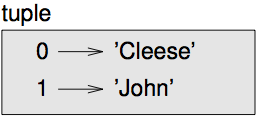
\includegraphics[scale=0.8]{figs/tuple1.pdf}}
\caption{State diagram.}
\label{fig.tuple1}
\end{figure}

But in a larger diagram you might want to leave out the
details.  For example, a diagram of the telephone directory might
appear as in Figure~\ref{fig.dict2}.

\begin{figure}
\centerline
{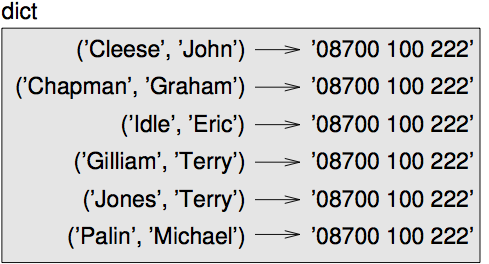
\includegraphics[scale=0.8]{figs/dict2.pdf}}
\caption{State diagram.}
\label{fig.dict2}
\end{figure}

Here the tuples are shown using Python syntax as a graphical
shorthand.

The telephone number in the diagram is the complaints line for the
BBC, so please don't call it.



\section{Comparing tuples}
\index{comparison!tuple}
\index{tuple!comparison}
\index{sort method}
\index{method!sort}

The relational operators work with tuples and other sequences;
Python starts by comparing the first element from each
sequence.  If they are equal, it goes on to the next elements,
and so on, until it finds elements that differ.  Subsequent
elements are not considered (even if they are really big).

\begin{verbatim}
>>> (0, 1, 2) < (0, 3, 4)
True
>>> (0, 1, 2000000) < (0, 3, 4)
True
\end{verbatim}
%
The {\tt sort} function works the same way.  It sorts 
primarily by first element, but in the case of a tie, it sorts
by second element, and so on.  

This feature lends itself to a pattern called {\bf DSU} for 

\begin{description}

\item[Decorate] a sequence by building a list of tuples
with one or more sort keys preceding the elements from the sequence,

\item[Sort] the list of tuples, and

\item[Undecorate] by extracting the sorted elements of the sequence.

\end{description}

\label{DSU}
\index{DSU pattern}
\index{pattern!DSU}
\index{decorate-sort-undecorate pattern}
\index{pattern!decorate-sort-undecorate}

For example, suppose you have a list of words and you want to
sort them from longest to shortest:

\begin{verbatim}
def sort_by_length(words):
    t = []
    for word in words:
       t.append((len(word), word))

    t.sort(reverse=True)

    res = []
    for length, word in t:
        res.append(word)
    return res
\end{verbatim}
%
The first loop builds a list of tuples, where each
tuple is a word preceded by its length.

{\tt sort} compares the first element, length, first, and
only considers the second element to break ties.  The keyword argument
{\tt reverse=True} tells {\tt sort} to go in decreasing order.
\index{keyword argument}
\index{argument!keyword}
\index{traversal}

The second loop traverses the list of tuples and builds a list of
words in descending order of length.

\begin{exercise}

In this example, ties are broken by comparing words, so words
with the same length appear in reverse alphabetical order.  For other
applications you might want to break ties at random.  Modify
this example so that words with the same length appear in
random order.  Hint: see the {\tt random} function in the
{\tt random} module.
Solution: \url{http://thinkpython.com/code/unstable_sort.py}.

\index{random module}
\index{module!random}
\index{random function}
\index{function!random}

\end{exercise}


\section{Sequences of sequences}
\index{sequence}

I have focused on lists of tuples, but almost all of the examples in
this chapter also work with lists of lists, tuples of tuples, and
tuples of lists.  To avoid enumerating the possible combinations, it
is sometimes easier to talk about sequences of sequences.

In many contexts, the different kinds of sequences (strings, lists and
tuples) can be used interchangeably.  So how and why do you choose one
over the others?
\index{string}
\index{list}
\index{tuple}
\index{mutability}
\index{immutability}

To start with the obvious, strings are more limited than other
sequences because the elements have to be characters.  They are
also immutable.  If you need the ability to change the characters
in a string (as opposed to creating a new string), you might
want to use a list of characters instead.

Lists are more common than tuples, mostly because they are mutable.
But there are a few cases where you might prefer tuples:

\begin{enumerate}

\item In some contexts, like a {\tt return} statement, it is
syntactically simpler to create a tuple than a list.  In other
contexts, you might prefer a list.

\item If you want to use a sequence as a dictionary key, you
have to use an immutable type like a tuple or string.

\item If you are passing a sequence as an argument to a function,
using tuples reduces the potential for unexpected behavior
due to aliasing.

\end{enumerate}

Because tuples are immutable, they don't provide methods
like {\tt sort} and {\tt reverse}, which modify existing lists.
But Python provides the built-in functions {\tt sorted}
and {\tt reversed}, which take any sequence as a parameter
and return a new list with the same elements in a different
order.
\index{sorted function}
\index{function!sorted}
\index{reversed function}
\index{function!reversed}


\section{Debugging}
\index{debugging}
\index{data structure}
\index{shape error}
\index{error!shape}

Lists, dictionaries and tuples are known generically as {\bf data
  structures}; in this chapter we are starting to see compound data
structures, like lists of tuples, and dictionaries that contain tuples
as keys and lists as values.  Compound data structures are useful, but
they are prone to what I call {\bf shape errors}; that is, errors
caused when a data structure has the wrong type, size or composition.
For example, if you are expecting a list with one integer and I
give you a plain old integer (not in a list), it won't work.
\index{structshape module}
\index{module!structshape}

% TODO: structshape is now part of Swampy

To help debug these kinds of errors, I have written a module
called {\tt structshape} that provides a function, also called
{\tt structshape}, that takes any kind of data structure as
an argument and returns a string that summarizes its shape.
You can download it from \url{http://thinkpython.com/code/structshape.py}

Here's the result for a simple list:

\begin{verbatim}
>>> from structshape import structshape
>>> t = [1,2,3]
>>> print structshape(t)
list of 3 int
\end{verbatim}
%
A fancier program might write ``list of 3 int{\em s},'' but it
was easier not to deal with plurals.  Here's a list of lists:

\begin{verbatim}
>>> t2 = [[1,2], [3,4], [5,6]]
>>> print structshape(t2)
list of 3 list of 2 int
\end{verbatim}
%
If the elements of the list are not the same type,
{\tt structshape} groups them, in order, by type:

\begin{verbatim}
>>> t3 = [1, 2, 3, 4.0, '5', '6', [7], [8], 9]
>>> print structshape(t3)
list of (3 int, float, 2 str, 2 list of int, int)
\end{verbatim}
%
Here's a list of tuples:

\begin{verbatim}
>>> s = 'abc'
>>> lt = zip(t, s)
>>> print structshape(lt)
list of 3 tuple of (int, str)
\end{verbatim}
%
And here's a dictionary with 3 items that map integers to strings.

\begin{verbatim}
>>> d = dict(lt) 
>>> print structshape(d)
dict of 3 int->str
\end{verbatim}
%
If you are having trouble keeping track of your data structures,
{\tt structshape} can help.


\section{Glossary}

\begin{description}

\item[tuple:] An immutable sequence of elements.
\index{tuple}

\item[tuple assignment:] An assignment with a sequence on the
right side and a tuple of variables on the left.  The right
side is evaluated and then its elements are assigned to the
variables on the left.
\index{tuple assignment}
\index{assignment!tuple}

\item[gather:] The operation of assembling a variable-length
argument tuple.
\index{gather}

\item[scatter:] The operation of treating a sequence as a list of
arguments.
\index{scatter}

\item[DSU:] Abbreviation of ``decorate-sort-undecorate,'' a
pattern that involves building a list of tuples, sorting, and
extracting part of the result.
\index{DSU pattern}

\item[data structure:] A collection of related values, often
organized in lists, dictionaries, tuples, etc.
\index{data structure}

\item[shape (of a data structure):] A summary of the type,
size and composition of a data structure.
\index{shape}

\end{description}


\section{Exercises}

\begin{exercise}

Write a function called \verb"most_frequent" that takes a string and
prints the letters in decreasing order of frequency.  Find text
samples from several different languages and see how letter frequency
varies between languages.  Compare your results with the tables at
\url{http://en.wikipedia.org/wiki/Letter_frequencies}.  Solution:
\url{http://thinkpython.com/code/most_frequent.py}.  \index{letter
  frequency} \index{frequency!letter}

\end{exercise}


\begin{exercise}
\label{anagrams}
\index{anagram set}
\index{set!anagram}

More anagrams!

\begin{enumerate}

\item Write a program
that reads a word list from a file (see Section~\ref{wordlist}) and
prints all the sets of words that are anagrams.

Here is an example of what the output might look like:

\begin{verbatim}
['deltas', 'desalt', 'lasted', 'salted', 'slated', 'staled']
['retainers', 'ternaries']
['generating', 'greatening']
['resmelts', 'smelters', 'termless']
\end{verbatim}
%
Hint: you might want to build a dictionary that maps from a
set of letters to a list of words that can be spelled with those
letters.  The question is, how can you represent the set of
letters in a way that can be used as a key?

\item Modify the previous program so that it prints the largest set
of anagrams first, followed by the second largest set, and so on.
\index{Scrabble}
\index{bingo}

\item In Scrabble a ``bingo'' is when you play all seven tiles in
your rack, along with a letter on the board, to form an eight-letter
word.  What set of 8 letters forms the most possible bingos?
Hint: there are seven.

% (7, ['angriest', 'astringe', 'ganister', 'gantries', 'granites',
% 'ingrates', 'rangiest'])

Solution: \url{http://thinkpython.com/code/anagram_sets.py}.

\end{enumerate}
\end{exercise}

\begin{exercise}
\index{metathesis}

Two words form a ``metathesis pair'' if you can transform one into the
other by swapping two letters; for example, ``converse'' and
``conserve.''  Write a program that finds all of the metathesis pairs
in the dictionary.  Hint: don't test all pairs of words, and don't
test all possible swaps.  Solution: \url{http://thinkpython.com/code/metathesis.py}.
Credit: This exercise is inspired by an example at \url{http://puzzlers.org}.

\end{exercise}



\begin{exercise}
\index{Car Talk}
\index{Puzzler}

Here's another Car Talk Puzzler
(\url{http://www.cartalk.com/content/puzzlers}):

\begin{quote}
What is the longest English word, that remains a valid English word,
as you remove its letters one at a time?

Now, letters can be removed from either end, or the middle, but you
can't rearrange any of the letters. Every time you drop a letter, you
wind up with another English word. If you do that, you're eventually
going to wind up with one letter and that too is going to be an
English word---one that's found in the dictionary. I want to know
what's the longest word and how many letters does it
have?

I'm going to give you a little modest example: Sprite. Ok? You start
off with sprite, you take a letter off, one from the interior of the
word, take the r away, and we're left with the word spite, then we
take the e off the end, we're left with spit, we take the s off, we're
left with pit, it, and I.
\end{quote}
\index{reducible word}
\index{word, reducible}

Write a program to find all words that can be reduced in this way,
and then find the longest one.

This exercise is a little more challenging than most, so here are
some suggestions:

\begin{enumerate}

\item You might want to write a function that takes a word and
  computes a list of all the words that can be formed by removing one
  letter.  These are the ``children'' of the word.
\index{recursive definition}
\index{definition!recursive}

\item Recursively, a word is reducible if any of its children
are reducible.  As a base case, you can consider the empty
string reducible.

\item The wordlist I provided, {\tt words.txt}, doesn't
contain single letter words.  So you might want to add
``I'', ``a'', and the empty string.

\item To improve the performance of your program, you might want
to memoize the words that are known to be reducible.

\end{enumerate}

Solution: \url{http://thinkpython.com/code/reducible.py}.

\end{exercise}




%\begin{exercise}
%\url{http://en.wikipedia.org/wiki/Word_Ladder}
%\end{exercise}





\section{Word frequency analysis}
\label{analysis}

As usual, you should at least attempt the following exercises
before you read my solutions.

\begin{exercise}

Write a program that reads a file, breaks each line into
words, strips whitespace and punctuation from the words, and
converts them to lowercase.
\index{string module}
\index{module!string}

Hint: The {\tt string} module provides strings named {\tt whitespace},
which contains space, tab, newline, etc., and {\tt
  punctuation} which contains the punctuation characters.  Let's see
if we can make Python swear:

\begin{verbatim}
>>> import string
>>> print string.punctuation
!"#$%&'()*+,-./:;<=>?@[\]^_`{|}~
\end{verbatim}
%
Also, you might consider using the string methods {\tt strip},
{\tt replace} and {\tt translate}.
\index{strip method}
\index{method!strip}
\index{replace method}
\index{method!replace}
\index{translate method}
\index{method!translate}

\end{exercise}


\begin{exercise}
\index{Project Gutenberg}

Go to Project Gutenberg (\url{http://gutenberg.org}) and download 
your favorite out-of-copyright book in plain text format.
\index{plain text}
\index{text!plain}

Modify your program from the previous exercise to read the book
you downloaded, skip over the header information at the beginning
of the file, and process the rest of the words as before.

Then modify the program to count the total number of words in
the book, and the number of times each word is used.
\index{word frequency}
\index{frequency!word}

Print the number of different words used in the book.  Compare
different books by different authors, written in different eras.
Which author uses the most extensive vocabulary?
\end{exercise}


\begin{exercise}

Modify the program from the previous exercise to print the
20 most frequently-used words in the book.

\end{exercise}


\begin{exercise}

Modify the previous program to read a word list (see
Section~\ref{wordlist}) and then print all the words in the book that
are not in the word list.  How many of them are typos?  How many of
them are common words that {\em should} be in the word list, and how
many of them are really obscure?

\end{exercise}


\section{Random numbers}
\index{random number}
\index{number, random}
\index{deterministic}
\index{pseudorandom}

Given the same inputs, most computer programs generate the same
outputs every time, so they are said to be {\bf deterministic}.
Determinism is usually a good thing, since we expect the same
calculation to yield the same result.  For some applications, though,
we want the computer to be unpredictable.  Games are an obvious
example, but there are more.

Making a program truly nondeterministic turns out to be not so easy,
but there are ways to make it at least seem nondeterministic.  One of
them is to use algorithms that generate {\bf pseudorandom} numbers.
Pseudorandom numbers are not truly random because they are generated
by a deterministic computation, but just by looking at the numbers it
is all but impossible to distinguish them from random.
\index{random module}
\index{module!random}

The {\tt random} module provides functions that generate
pseudorandom numbers (which I will simply call ``random'' from
here on).
\index{random function}
\index{function!random}

The function {\tt random} returns a random float
between 0.0 and 1.0 (including 0.0 but not 1.0).  Each time you
call {\tt random}, you get the next number in a long series.  To see a
sample, run this loop:

\begin{verbatim}
import random

for i in range(10):
    x = random.random()
    print x
\end{verbatim}
%
The function {\tt randint} takes parameters {\tt low} and
{\tt high} and returns an integer between {\tt low} and
{\tt high} (including both).
\index{randint function}
\index{function!randint}

\begin{verbatim}
>>> random.randint(5, 10)
5
>>> random.randint(5, 10)
9
\end{verbatim}
%
To choose an element from a sequence at random, you can use
{\tt choice}:
\index{choice function}
\index{function!choice}

\begin{verbatim}
>>> t = [1, 2, 3]
>>> random.choice(t)
2
>>> random.choice(t)
3
\end{verbatim}
%
The {\tt random} module also provides functions to generate
random values from continuous distributions including
Gaussian, exponential, gamma, and a few more.

\begin{exercise}
\index{histogram!random choice}

Write a function named \verb"choose_from_hist" that takes
a histogram as defined in Section~\ref{histogram} and returns a 
random value from the histogram, chosen with probability
in proportion to frequency.  For example, for this histogram:

\begin{verbatim}
>>> t = ['a', 'a', 'b']
>>> hist = histogram(t)
>>> print hist
{'a': 2, 'b': 1}
\end{verbatim}
%
your function should return {\tt 'a'} with probability $2/3$ and {\tt 'b'}
with probability $1/3$.
\end{exercise}


\section{Word histogram}

You should attempt the previous exercises before you go on.
You can download my solution from
 \url{http://thinkpython.com/code/analyze_book.py}.  You will
also need \url{http://thinkpython.com/code/emma.txt}.

Here is a program that reads a file and builds a histogram of the
words in the file:
\index{histogram!word frequencies}

\begin{verbatim}
import string

def process_file(filename):
    hist = dict()
    fp = open(filename)
    for line in fp:
        process_line(line, hist)
    return hist

def process_line(line, hist):
    line = line.replace('-', ' ')
    
    for word in line.split():
        word = word.strip(string.punctuation + string.whitespace)
        word = word.lower()

        hist[word] = hist.get(word, 0) + 1

hist = process_file('emma.txt')
\end{verbatim}
%
This program reads {\tt emma.txt}, which contains the text of {\em
  Emma} by Jane Austen.
\index{Austin, Jane}

\verb"process_file" loops through the lines of the file,
passing them one at a time to \verb"process_line".  The histogram
{\tt hist} is being used as an accumulator.
\index{accumulator!histogram}
\index{traversal}

\verb"process_line" uses the string method {\tt replace} to replace
hyphens with spaces before using {\tt split} to break the line into a
list of strings.  It traverses the list of words and uses {\tt strip}
and {\tt lower} to remove punctuation and convert to lower case.  (It
is a shorthand to say that strings are ``converted;'' remember that
string are immutable, so methods like {\tt strip} and {\tt lower}
return new strings.)

Finally, \verb"process_line" updates the histogram by creating a new
item or incrementing an existing one.
\index{update!histogram}

To count the total number of words in the file, we can add up
the frequencies in the histogram:

\begin{verbatim}
def total_words(hist):
    return sum(hist.values())
\end{verbatim}
%
The number of different words is just the number of items in
the dictionary:

\begin{verbatim}
def different_words(hist):
    return len(hist)
\end{verbatim}
%
Here is some code to print the results:

\begin{verbatim}
print 'Total number of words:', total_words(hist)
print 'Number of different words:', different_words(hist)
\end{verbatim}
%
And the results:

\begin{verbatim}
Total number of words: 161080
Number of different words: 7214
\end{verbatim}
%

\section{Most common words}
\index{DSU pattern}
\index{pattern!DSU}

To find the most common words, we can apply the DSU pattern;
\verb"most_common" takes a histogram and returns a list of
word-frequency tuples, sorted in reverse order by frequency:

\begin{verbatim}
def most_common(hist):
    t = []
    for key, value in hist.items():
        t.append((value, key))

    t.sort(reverse=True)
    return t
\end{verbatim}
%
Here is a loop that prints the ten most common words:

\begin{verbatim}
t = most_common(hist)
print 'The most common words are:'
for freq, word in t[0:10]:
    print word, '\t', freq
\end{verbatim}
%
And here are the results from {\em Emma}:

\begin{verbatim}
The most common words are:
to 	5242
the 	5205
and 	4897
of 	4295
i 	3191
a 	3130
it 	2529
her 	2483
was 	2400
she 	2364
\end{verbatim}
%

\section{Optional parameters}
\index{optional parameter}
\index{parameter!optional}

We have seen built-in functions and methods that take a variable
number of arguments.  It is possible to write user-defined functions
with optional arguments, too.  For example, here is a function that
prints the most common words in a histogram

\begin{verbatim}
def print_most_common(hist, num=10):
    t = most_common(hist)
    print 'The most common words are:'
    for freq, word in t[:num]:
        print word, '\t', freq
\end{verbatim}

The first parameter is required; the second is optional.
The {\bf default value} of {\tt num} is 10.
\index{default value}
\index{value!default}

If you only provide one argument:

\begin{verbatim}
print_most_common(hist)
\end{verbatim}

{\tt num} gets the default value.  If you provide two arguments:

\begin{verbatim}
print_most_common(hist, 20)
\end{verbatim}

{\tt num} gets the value of the argument instead.  In other
words, the optional argument {\bf overrides} the default value.
\index{override}

If a function has both required and optional parameters, all
the required parameters have to come first, followed by the
optional ones.


\section{Dictionary subtraction}
\index{dictionary!subtraction}
\index{subtraction!dictionary}

Finding the words from the book that are not in the word list
from {\tt words.txt} is a problem you might recognize as set
subtraction; that is, we want to find all the words from one
set (the words in the book) that are not in another set (the
words in the list).

{\tt subtract} takes dictionaries {\tt d1} and {\tt d2} and returns a
new dictionary that contains all the keys from {\tt d1} that are not
in {\tt d2}.  Since we don't really care about the values, we
set them all to None.

\begin{verbatim}
def subtract(d1, d2):
    res = dict()
    for key in d1:
        if key not in d2:
            res[key] = None
    return res
\end{verbatim}
%
To find the words in the book that are not in {\tt words.txt},
we can use \verb"process_file" to build a histogram for
{\tt words.txt}, and then subtract:

\begin{verbatim}
words = process_file('words.txt')
diff = subtract(hist, words)

print "The words in the book that aren't in the word list are:"
for word in diff.keys():
    print word,
\end{verbatim}
%
Here are some of the results from {\em Emma}:

\begin{verbatim}
The words in the book that aren't in the word list are:
 rencontre jane's blanche woodhouses disingenuousness 
friend's venice apartment ...
\end{verbatim}
%
Some of these words are names and possessives.  Others, like
``rencontre,'' are no longer in common use.  But a few are common
words that should really be in the list!

\begin{exercise}
\index{set}
\index{type!set}

Python provides a data structure called {\tt set} that provides many
common set operations.  Read the documentation at
\url{http://docs.python.org/2/library/stdtypes.html#types-set} and
write a program that uses set subtraction to find words in the book
that are not in the word list.  Solution:
\url{http://thinkpython.com/code/analyze_book2.py}.

\end{exercise}


\section{Random words}
\label{randomwords}
\index{histogram!random choice}

To choose a random word from the histogram, the simplest algorithm
is to build a list with multiple copies of each word, according
to the observed frequency, and then choose from the list:

\begin{verbatim}
def random_word(h):
    t = []
    for word, freq in h.items():
        t.extend([word] * freq)

    return random.choice(t)
\end{verbatim}
%
The expression {\tt [word] * freq} creates a list with {\tt freq}
copies of the string {\tt word}.  The {\tt extend}
method is similar to {\tt append} except that the argument is
a sequence.

\begin{exercise}
\label{randhist}
\index{algorithm}

This algorithm works, but it is not very efficient; each time you
choose a random word, it rebuilds the list, which is as big as
the original book.  An obvious improvement is to build the list
once and then make multiple selections, but the list is still big.

An alternative is:

\begin{enumerate}

\item Use {\tt keys} to get a list of the words in the book.

\item Build a list that contains the cumulative sum of the word
  frequencies (see Exercise~\ref{cumulative}).  The last item
  in this list is the total number of words in the book, $n$.
  
\item Choose a random number from 1 to $n$.  Use a bisection search
  (See Exercise~\ref{bisection}) to find the index where the random
  number would be inserted in the cumulative sum.

\item Use the index to find the corresponding word in the word list.

\end{enumerate}

Write a program that uses this algorithm to choose a random
word from the book.  Solution: \url{http://thinkpython.com/code/analyze_book3.py}.

\end{exercise}



\section{Markov analysis}
\label{markov}
\index{Markov analysis}

If you choose words from the book at random, you can get a
sense of the vocabulary, you probably won't get a sentence:

\begin{verbatim}
this the small regard harriet which knightley's it most things
\end{verbatim}
%
A series of random words seldom makes sense because there
is no relationship between successive words.  For example, in
a real sentence you would expect an article like ``the'' to
be followed by an adjective or a noun, and probably not a verb
or adverb.

One way to measure these kinds of relationships is Markov
analysis, which
characterizes, for a given sequence of words, the probability of the
word that comes next.  For example, the song {\em Eric, the Half a
  Bee} begins:

\begin{quote}
Half a bee, philosophically, \\
Must, ipso facto, half not be. \\
But half the bee has got to be \\
Vis a vis, its entity. D'you see? \\
\\
But can a bee be said to be \\
Or not to be an entire bee \\
When half the bee is not a bee \\
Due to some ancient injury? \\
\end{quote}
%
In this text,
the phrase ``half the'' is always followed by the word ``bee,''
but the phrase ``the bee'' might be followed by either
``has'' or ``is''.
\index{prefix}
\index{suffix}
\index{mapping}

The result of Markov analysis is a mapping from each prefix
(like ``half the'' and ``the bee'') to all possible suffixes
(like ``has'' and ``is'').
\index{random text}
\index{text!random}

Given this mapping, you can generate a random text by
starting with any prefix and choosing at random from the
possible suffixes.  Next, you can combine the end of the
prefix and the new suffix to form the next prefix, and repeat.

For example, if you start with the prefix ``Half a,'' then the
next word has to be ``bee,'' because the prefix only appears
once in the text.  The next prefix is ``a bee,'' so the
next suffix might be ``philosophically,'' ``be'' or ``due.''

In this example the length of the prefix is always two, but
you can do Markov analysis with any prefix length.  The length
of the prefix is called the ``order'' of the analysis.

\begin{exercise}

Markov analysis:

\begin{enumerate}

\item Write a program to read a text from a file and perform Markov
analysis.  The result should be a dictionary that maps from
prefixes to a collection of possible suffixes.  The collection
might be a list, tuple, or dictionary; it is up to you to make
an appropriate choice.  You can test your program with prefix
length two, but you should write the program in a way that makes
it easy to try other lengths.

\item Add a function to the previous program to generate random text
based on the Markov analysis.  Here is an example from {\em Emma}
with prefix length 2:

\begin{quote}
He was very clever, be it sweetness or be angry, ashamed or only
amused, at such a stroke. She had never thought of Hannah till you
were never meant for me?" "I cannot make speeches, Emma:" he soon cut
it all himself.
\end{quote}

For this example, I left the punctuation attached to the words.
The result is almost syntactically correct, but not quite.
Semantically, it almost makes sense, but not quite.

What happens if you increase the prefix length?  Does the random
text make more sense?
\index{mash-up}

\item Once your program is working, you might want to try a mash-up:
if you analyze text from two or more books, the random
text you generate will blend the vocabulary and phrases from
the sources in interesting ways.

\end{enumerate}

Credit: This case study is based on an example from Kernighan and
Pike, {\em The Practice of Programming}, Addison-Wesley, 1999.

\end{exercise}

You should attempt this exercise before you go on; then you can can
download my solution from \url{http://thinkpython.com/code/markov.py}.  You
will also need \url{http://thinkpython.com/code/emma.txt}.


\section{Data structures}
\index{data structure}

Using Markov analysis to generate random text is fun, but there is
also a point to this exercise: data structure selection.  In your
solution to the previous exercises, you had to choose:

\begin{itemize}

\item How to represent the prefixes.

\item How to represent the collection of possible suffixes.

\item How to represent the mapping from each prefix to
the collection of possible suffixes.

\end{itemize}

Ok, the last one is easy; the only mapping type we have
seen is a dictionary, so it is the natural choice.

For the prefixes, the most obvious options are string,
list of strings, or tuple of strings.  For the suffixes,
one option is a list; another is a histogram (dictionary).
\index{implementation}

How should you choose?  The first step is to think about
the operations you will need to implement for each data structure.
For the prefixes, we need to be able to remove words from
the beginning and add to the end.  For example, if the current
prefix is ``Half a,'' and the next word is ``bee,'' you need
to be able to form the next prefix, ``a bee.''
\index{tuple!as key in dictionary}

Your first choice might be a list, since it is easy to add
and remove elements, but we also need to be able to use the
prefixes as keys in a dictionary, so that rules out lists.
With tuples, you can't append or remove, but you can use
the addition operator to form a new tuple:

\begin{verbatim}
def shift(prefix, word):
    return prefix[1:] + (word,)
\end{verbatim}
%
{\tt shift} takes a tuple of words, {\tt prefix}, and a string, 
{\tt word}, and forms a new tuple that has all the words
in {\tt prefix} except the first, and {\tt word} added to
the end.

For the collection of suffixes, the operations we need to
perform include adding a new suffix (or increasing the frequency
of an existing one), and choosing a random suffix.

Adding a new suffix is equally easy for the list implementation
or the histogram.  Choosing a random element from a list
is easy; choosing from a histogram is harder to do
efficiently (see Exercise~\ref{randhist}).

So far we have been talking mostly about ease of implementation,
but there are other factors to consider in choosing data structures.
One is run time.  Sometimes there is a theoretical reason to expect
one data structure to be faster than other; for example, I mentioned
that the {\tt in} operator is faster for dictionaries than for lists,
at least when the number of elements is large.

But often you don't know ahead of time which implementation will
be faster.  One option is to implement both of them and see which
is better.  This approach is called {\bf benchmarking}.  A practical
alternative is to choose the data structure that is
easiest to implement, and then see if it is fast enough for the
intended application.  If so, there is no need to go on.  If not,
there are tools, like the {\tt profile} module, that can identify
the places in a program that take the most time.
\index{benchmarking}
\index{profile module}
\index{module!profile}

The other factor to consider is storage space.  For example, using a
histogram for the collection of suffixes might take less space because
you only have to store each word once, no matter how many times it
appears in the text.  In some cases, saving space can also make your
program run faster, and in the extreme, your program might not run at
all if you run out of memory.  But for many applications, space is a
secondary consideration after run time.

One final thought: in this discussion, I have implied that
we should use one data structure for both analysis and generation.  But
since these are separate phases, it would also be possible to use one
structure for analysis and then convert to another structure for
generation.  This would be a net win if the time saved during
generation exceeded the time spent in conversion.


\section{Debugging}
\index{debugging}

When you are debugging a program, and especially if you are
working on a hard bug, there are four things to try:

\begin{description}

\item[reading:] Examine your code, read it back to yourself, and
check that it says what you meant to say.

\item[running:] Experiment by making changes and running different
versions.  Often if you display the right thing at the right place
in the program, the problem becomes obvious, but sometimes you have to
spend some time to build scaffolding.

\item[ruminating:] Take some time to think!  What kind of error
is it: syntax, runtime, semantic?  What information can you get from
the error messages, or from the output of the program?  What kind of
error could cause the problem you're seeing?  What did you change
last, before the problem appeared?

\item[retreating:] At some point, the best thing to do is back
off, undoing recent changes, until you get back to a program that
works and that you understand.  Then you can start rebuilding.

\end{description}

Beginning programmers sometimes get stuck on one of these activities
and forget the others.  Each activity comes with its own failure
mode.
\index{typographical error}

For example, reading your code might help if the problem is a
typographical error, but not if the problem is a conceptual
misunderstanding.  If you don't understand what your program does, you
can read it 100 times and never see the error, because the error is in
your head.
\index{experimental debugging}

Running experiments can help, especially if you run small, simple
tests.  But if you run experiments without thinking or reading your
code, you might fall into a pattern I call ``random walk programming,''
which is the process of making random changes until the program
does the right thing.  Needless to say, random walk programming
can take a long time.
\index{random walk programming}
\index{development plan!random walk programming}

You have to take time to think.  Debugging is like an
experimental science.  You should have at least one hypothesis about
what the problem is.  If there are two or more possibilities, try to
think of a test that would eliminate one of them.

Taking a break helps with the thinking.  So does talking.
If you explain the problem to someone else (or even yourself), you
will sometimes find the answer before you finish asking the question.

But even the best debugging techniques will fail if there are too many
errors, or if the code you are trying to fix is too big and
complicated.  Sometimes the best option is to retreat, simplifying the
program until you get to something that works and that you
understand.

Beginning programmers are often reluctant to retreat because
they can't stand to delete a line of code (even if it's wrong).
If it makes you feel better, copy your program into another file
before you start stripping it down.  Then you can paste the pieces
back in a little bit at a time.

Finding a hard bug requires reading, running, ruminating, and
sometimes retreating.  If you get stuck on one of these activities,
try the others.


\section{Glossary}

\begin{description}

\item[deterministic:] Pertaining to a program that does the same
thing each time it runs, given the same inputs.
\index{deterministic}

\item[pseudorandom:] Pertaining to a sequence of numbers that appear
to be random, but are generated by a deterministic program.
\index{pseudorandom}

\item[default value:] The value given to an optional parameter if no
argument is provided.
\index{default value}

\item[override:] To replace a default value with an argument.
\index{override}

\item[benchmarking:] The process of choosing between data structures
by implementing alternatives and testing them on a sample of the
possible inputs.  
\index{benchmarking}

\end{description}


\section{Exercises}

\begin{exercise}
\index{word frequency}
\index{frequency!word}
\index{Zipf's law}

The ``rank'' of a word is its position in a list of words
sorted by frequency: the most common word has rank 1, the
second most common has rank 2, etc.

Zipf's law describes a relationship between the ranks and frequencies
of words in natural languages
(\url{http://en.wikipedia.org/wiki/Zipf's_law}).  Specifically, it
predicts that the frequency, $f$, of the word with rank $r$ is:

\[ f = c r^{-s} \]
%
where $s$ and $c$ are parameters that depend on the language and the
text.  If you take the logarithm of both sides of this equation, you
get:
\index{logarithm}

\[ \log f = \log c - s \log r \]
%
So if you plot log $f$ versus log $r$, you should get
a straight line with slope $-s$ and intercept log $c$.

Write a program that reads a text from a file, counts
word frequencies, and prints one line
for each word, in descending order of frequency, with
log $f$ and log $r$.  Use the graphing program of your
choice to plot the results and check whether they form
a straight line.  Can you estimate the value of $s$?

Solution: \url{http://thinkpython.com/code/zipf.py}.  To make the plots, you
might have to install matplotlib (see
\url{http://matplotlib.sourceforge.net/}).
\index{Matplotlib}

\end{exercise}


